\documentclass[11pt]{article}

\usepackage[bottom]{footmisc}

\usepackage{xcolor}

\usepackage{amsthm}
\usepackage{amssymb}
\usepackage{amsmath}

\usepackage{mathtools}

\usepackage{hyperref}

\usepackage{caption}
\usepackage{subcaption}

\usepackage{xepersian}

\settextfont{Adobe Arabic}
\setlatintextfont[Scale= 0.85]{Times New Roman}


\title{گزارش پروژه‌ی شبیه سازی 1 احتمال}
\author{آریا ادیبی ۹۲۱۱۰۴۷۶}
\date{}

\definecolor{darkishBlue}{RGB}{27, 71, 188}

\hypersetup{
	colorlinks= true,
	linkcolor= darkishBlue,
%	anchorcolor= black,
	citecolor= black,
%	filecolor= cyan,
%	menucolor= red,
%	runcolor= cyan,
	urlcolor= darkishBlue,
%	allcolors= black
}

\setcounter{secnumdepth}{0}

\theoremstyle{definition}
\newtheorem*{definition}{تعریف}

\theoremstyle{lemma}
\newtheorem*{lemma}{لم}

\theoremstyle{remark}
\newtheorem*{remark}{ملاحضه}

\renewcommand\qedsymbol{\rule{0.2cm}{0.2cm}}

\begin{document}
	\maketitle
	
	 قبل از هر چیز ذکر چند نکته ضروری است:
	 \begin{itemize}
	 	\item
	 	اسمی که خواسته شده بود برای فایل‌های کد خود بگذاریم اسمی استاندارد نبود و من به دلیل
	 	این که مشکلی پیش نیاید یا حداقل «اخطار» این موضوع را نبینم این اسم را به
	 	\lr{qi\_studentNumber.m}
	 	تغییر دادم که در آن
	 	\lr{i}
	 	شماره‌ی پرسش است.
	 	
	 	\item
	 	کامپیوتر من قدرت نسبتاً زیادی دارد از این رو نمی‌دانستم که شمار آزمایش‌ها یا متغیر‌های 
	 	مربوط دیگر را چقدر بگذارم که از کامپوتر مقصد زمان زیادی نگیرد. از این رو در هر کد 
	 	قسمتی به نام
	 	\lr{initialization}
	 	قرار گرفته که بتوان تمامی متغیر‌های لازم پرسش را به مقدار دلخواه عوض کرد. این انعطاف
	 	بیشتری هم به کد می‌دهد. برخی از پرسش‌ها هم شمار آزمایش‌ها را بیشتر از شمار گفته شده
	 	گذاشتم که نتیجه‌ی بهتری به دست آید. اگر لازم دیدید در همین قسمت به شمار دلخواه تغییر دهید.
	 	
	 	\item
	 	متغیر‌های کد‌ها به گونه‌ای اسم گذاری و «توضیح» گذاری شده‌اند که کد به راحتی قابل فهم باشد
	 	از این رو آن‌ها را زیاد توضیح نمی‌دهم.
	 \end{itemize}
 	
 	%%%%%%%%%%%%%%%%%%%%%%%%%%%%%%%%%%%%%
 	\section{پرسش ۱ - تطابق تولد‌ها!}
 	کد روشن است و به خوبی «توضیح» گذاری شده است. تنها نکته‌ای که است این است که برای پیدا کردن
 	کمینه‌ی 
 	$n$
 	به طوری که احتمال مورد نظر بیشتر مساوی 
 	\lr{۰.۹}
 	شود از الگوریتم جست‌وجوی دودویی استفاده شده است.
 	همچنین در این کد زمان حساب هر بخش هم چاپ می‌شود که اگر خواستید حذف کنید.
 	
 	جواب‌های خواسته شده را با اجرا کردن کد ببینید. 
 	نمودار‌های حاصل را می‌توانید در
 	\textcolor{darkishBlue}{شکل}
 	\ref{q1}
 	ببینید.
	%%%%%%%%%%%%%%%%%%%%%%%%%%%%%%%%%%%%%
	\section{پرسش ۲ - در‌های جادویی}
	این پرسش نیز نام گذاری متغیر‌ها و «توضیح» گزاری‌ها کد را روشن می‌کند. برای دیدن جواب
	کد را اجرا کنید.
	نتیجه‌ای که می‌گیریم این است که استدلال ما برای پرسش مشهور
	\lr{ \textsc{TV game show} }
	درست بود. یعنی احتمال بودن جایزه پشت آن پرده‌ای که حذف نشده و توسط ما انتخاب نشده 
	برابر 
	$2/3$
	و این احتمال برای پرده‌ی انتخاب شده 
	$1/3$
	است. از این رو عاقلانس که پرده‌ی خود را عوض کنیم.
	%%%%%%%%%%%%%%%%%%%%%%%%%%%%%%%%%%%%%
	\section{پرسش ۳ - علی بی‌کار و سکه‌های پرتاب شونده}
	این پرسش نیز نام گذاری متغیر‌ها و «توضیح» گزاری‌ها کد را روشن می‌کند. برای دیدن جواب
	کد را اجرا کنید.
	
	برای حدس نظری این عدد آزمایش پرتاب سکه را در نظر بگیرید تا خط بیاید («موفقیت»). متغیر
	تصادفی 
	$X$
	هندسی را به طور معمول تعریف کنید. داریم
	\begin{flalign*}
		P(X \ge r)	&= \sum_{i=r}^{\infty} (1-p)^i-1 \times p &\\
					&= \sum_{i=r}^{\infty} (1/2)^i=\ (\frac{1}{2})^{r-1}
	\end{flalign*}
	
	با این که در آزمایش اصلی این کمینه
	$r$
	تا شیر پشت سر هم می‌تواند جا‌های مختلفی بیاید ولی چون ۵۰ عدد بزرگی نیست این آزمایش
	تقریب خیلی بدی نخواهد بود. برای 
	$r=6$
	خواهیم که احتمال کمینه 
	$r$تا
	شیر پشت هم بیاید
	$\frac{1}{32}$
	است که عدد کمی است. از این رو حدس می‌زنم که شمار مورد انظار ما 
	\lr{(E)}
	کمتر مساوی ۶ باشد.
	%%%%%%%%%%%%%%%%%%%%%%%%%%%%%%%%%%%%%
	\section{پرسش ۴ - امید دگرگون}
	این پرسش نیز نام گذاری متغیر‌ها و «توضیح» گزاری‌ها کد را روشن می‌کند. برای دیدن جواب
	کد را اجرا کنید.
	
	دلیل درستی عبارت به صورا زیر است:
	\begin{flalign*}
		&P(X \ge r)= \sum_{i=r}^{\infty} P(X=i) & \\
		&\Rightarrow & \\
		&\sum_{i=1}^{\infty} P(X \ge i)=\ \sum_{i=1}^{\infty} iP(X=i)=\ 
		\sum_{x \in A} xP(X=x)=\ E(X) & \\
	\end{flalign*}
	%%%%%%%%%%%%%%%%%%%%%%%%%%%%%%%%%%%%%
	\section{پرسش ۵ - غار‌های شرطی}
	\begin{itemize}
		\item
		در این پرسش فرض کردم اگر در درست انخاب شود بلافاصله بیرون می‌رویم.
	\end{itemize}
	
	این پرسش نیز نام گذاری متغیر‌ها و «توضیح» گزاری‌ها کد را روشن می‌کند. برای دیدن جواب
	کد را اجرا کنید.
	%%%%%%%%%%%%%%%%%%%%%%%%%%%%%%%%%%%%%
	\section{پرسش ۶ - توضیع مشترک دوگانه}
	رابطه‌ی گفته شده
	\lr{ \textsc{Law of Unconscious Statistician} }
	است. اگر شمار متغیر‌های تصادفی ۱ باشد اثبات ‌آن در کتاب آقای قهرمانی آورده شده است.
	من اثبات را برای ۲ متغیر تصادفی می‌آورم. اثبات برای شمار بیشتری متغیر تصادفی کاملاً 
	مشابه است و من این کار را کردم که اثبات بدون دلیل شلوغ نشود.
	\begin{definition}
		تابع
		$f_{XY}$
		را تابع احتمال توأم متغیر‌های تصادفی
		$X$
		و
		$Y$
		بگیرید.
	\end{definition}
		
	\begin{definition}
		متغیر تصادفی
		$Z$
		را برابر 
		$Z= h(X,Y)$
		بگیرید.
	\end{definition}

	می‌دانیم برای تمامی 
	$z \in \text{Domain} (Z)$
	خواهیم داشت:
	\begin{flalign*}
		f_Z(z)	&=\ P(Z=z)&\\
				&=\ \sum_{ \{(x,y)| h(x,y)=z\} } f_{XY}(x, y)
	\end{flalign*}
	
	\begin{definition}
		به ازای هر 
		$z \in \text{Domain} (Z)$
		بگیرید:
		$A(z)=\ \{(x,y)| h(x,y)=z\}$
	\end{definition}
	
	با تعریف‌ها و نکته‌ی گفته شده خواهیم داشت:
	\begin{flalign*}
		E[Z] 	&= \sum_{z} zf_Z(z)&\\
				&= \sum_{z} \sum_{A(z)} h(x,y)f_{XY}(x,y)&\\
	\end{flalign*}
	این دو جمع معادل جمع روی تمام
	$(x, y)$های
	ممکن است. پس:

	$$E[Z]=\ \sum_{(x,y)} h(x,y)f_{XY}(x,y)$$
	دقیقاً همان چیزی که می‌خواستیم. 
	$\qed$
	
	این پرسش نیز نام گذاری متغیر‌ها و «توضیح» گزاری‌ها کد را روشن می‌کند. برای دیدن جواب
	کد را اجرا کنید. خواهید دید که این ۲ مقدار را یکی تشخیص می‌دهد.
	
	نمودار‌های حاصل را می‌توانید در 
	\textcolor{darkishBlue}{شکل}
	\ref{q6}
	ببینید.
	%%%%%%%%%%%%%%%%%%%%%%%%%%%%%%%%%%%%%
	\section{پرسش ۷ - مجموع}
	طبق قضیه‌ی حد مرکزی حدس این است که با بیشتر شدن
	$n$
	رفتاری مشابه‌تر متغیر تصادفی نرمال داشته باشیم. که همانگونه که می‌بینیم 
	همینگونه است.
	
	این پرسش نیز نام گذاری متغیر‌ها و «توضیح» گزاری‌ها کد را روشن می‌کند. برای دیدن جواب
	کد را اجرا کنید. 
	
	برخی از نمودار‌های خاصل را می‌توانید در 
	\textcolor{darkishBlue}{شکل}
	\ref{q7}
	ببینید.
	%%%%%%%%%%%%%%%%%%%%%%%%%%%%%%%%%%%%%
	%% 1
	\begin{figure}[h!]
		\centering
		\begin{subfigure}[h!]{0.48\textwidth}
			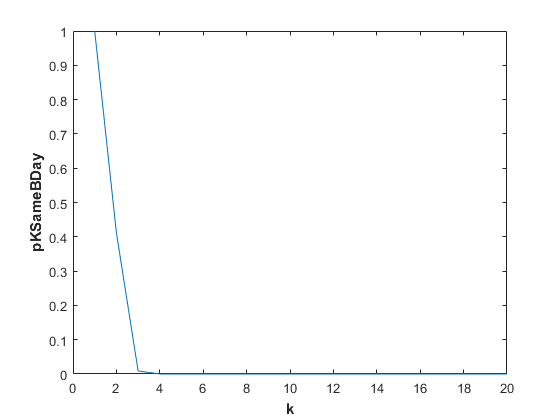
\includegraphics[width=\textwidth]{./Images/1/1.png}
			\caption{ \lr{pKSameBDay vs K -- n= 20} }
		\end{subfigure}
		\quad
		\begin{subfigure}[h!]{0.48\textwidth}
			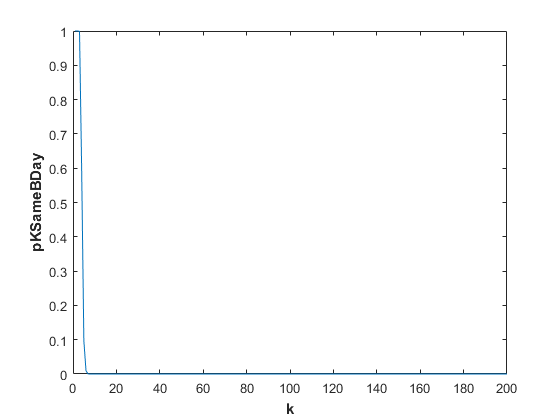
\includegraphics[width=\textwidth]{./Images/1/2.png}
			\caption{ \lr{pKSameBDay vs K -- n= 200} }
		\end{subfigure}
		
		\begin{subfigure}[h!]{0.48\textwidth}
			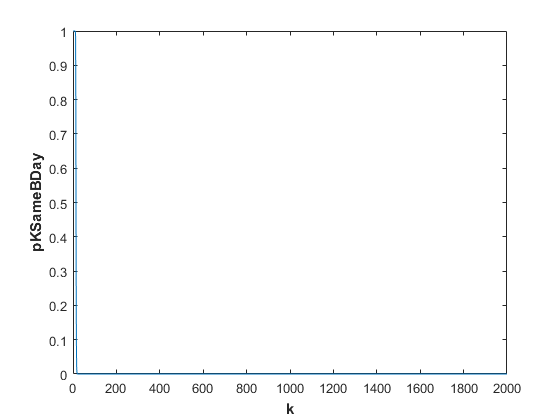
\includegraphics[width=\textwidth]{./Images/1/3.png}
			\caption{ \lr{pKSameBDay vs K -- n= 2000} }
		\end{subfigure}
		
		\caption{نمودار‌های پرسش ۱}
		\label{q1}
	\end{figure}
	
	%% 6
	\begin{figure}[h!]
		\centering
		\begin{subfigure}[h!]{0.48\textwidth}
			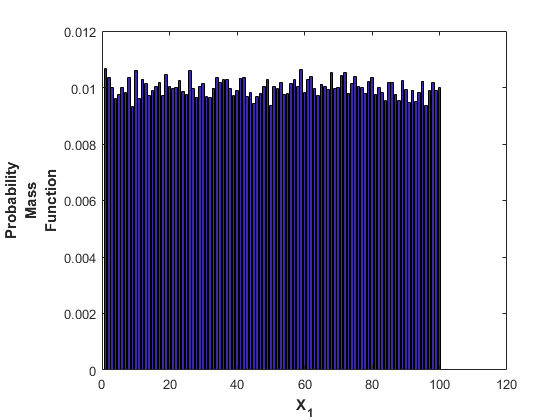
\includegraphics[width=\textwidth]{./Images/6/1.png}
			\caption{ \lr{Probability mass function $X_1$} }
		\end{subfigure}
		\quad
		\begin{subfigure}[h!]{0.48\textwidth}
			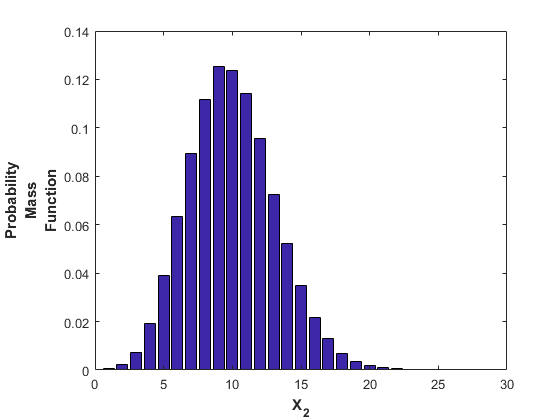
\includegraphics[width=\textwidth]{./Images/6/2.png}
			\caption{ \lr{Probability mass function $X_2$} }
		\end{subfigure}
		
		\begin{subfigure}[h!]{0.48\textwidth}
			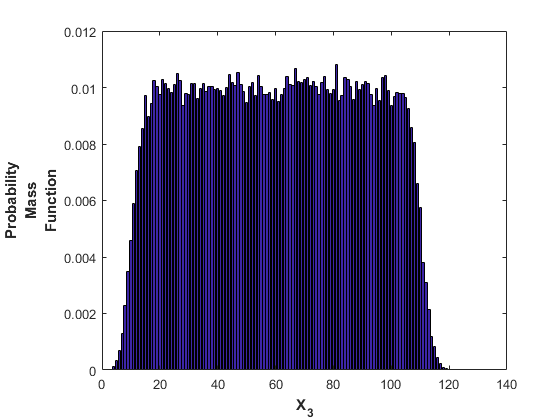
\includegraphics[width=\textwidth]{./Images/6/3.png}
			\caption{ \lr{Probability mass function $X_3$} }
		\end{subfigure}
		\quad
		\begin{subfigure}[h!]{0.48\textwidth}
			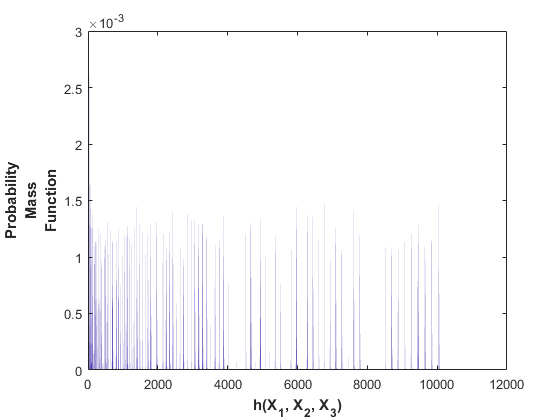
\includegraphics[width=\textwidth]{./Images/6/4.png}
			\caption{ \lr{Probability mass function $h(X_1, X_2, X_3)$} }
		\end{subfigure}
		\caption{نمودار‌های پرسش ۶}
		\label{q6}
	\end{figure}

	%% 7
	\begin{figure}[h!]
		\centering
		\begin{subfigure}[h!]{0.48\textwidth}
			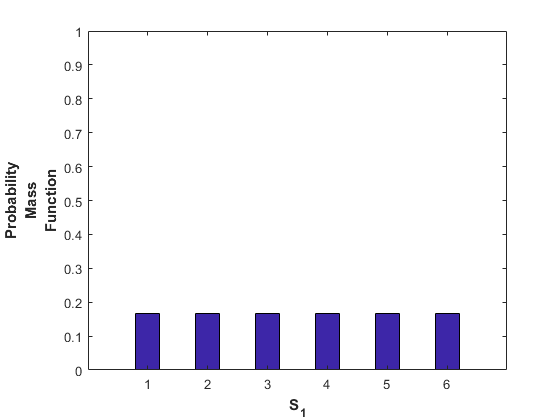
\includegraphics[width=\textwidth]{./Images/7/1.png}
			\caption{ $n=1$ }
		\end{subfigure}
		\quad
		\begin{subfigure}[h!]{0.48\textwidth}
			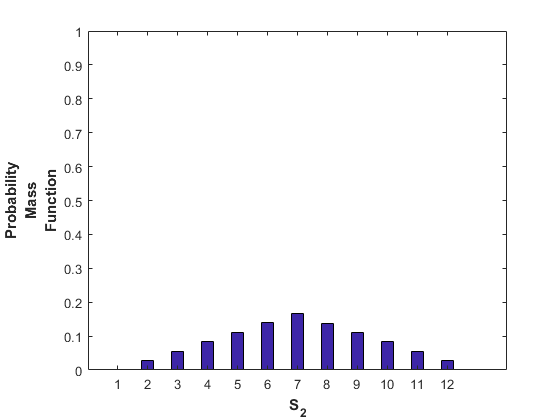
\includegraphics[width=\textwidth]{./Images/7/2.png}
			\caption{ $n=2$ }
		\end{subfigure}
		
		\begin{subfigure}[h!]{0.48\textwidth}
			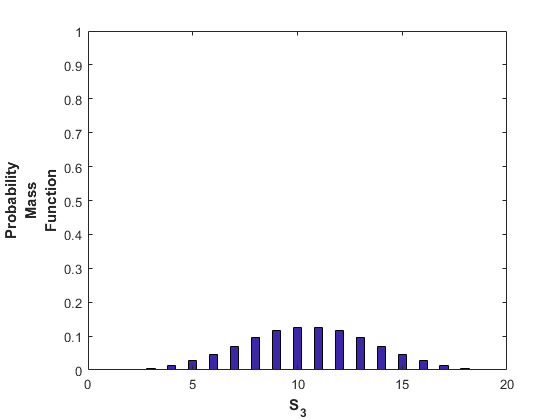
\includegraphics[width=\textwidth]{./Images/7/3.png}
			\caption{ $n=3$ }
		\end{subfigure}
		\quad
		\begin{subfigure}[h!]{0.48\textwidth}
			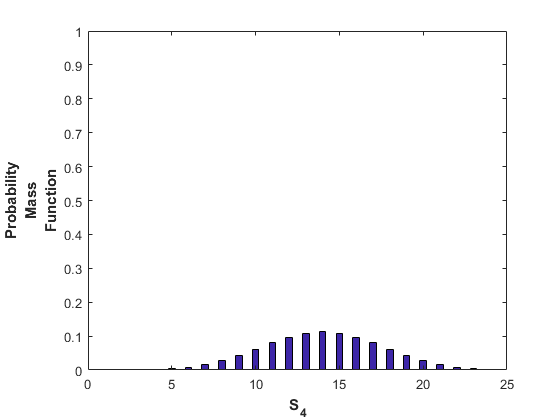
\includegraphics[width=\textwidth]{./Images/7/4.png}
			\caption{ $n=4$ }
		\end{subfigure}
	
		\begin{subfigure}[h!]{0.48\textwidth}
			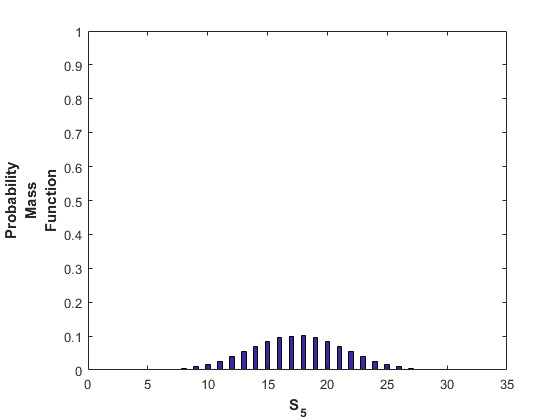
\includegraphics[width=\textwidth]{./Images/7/5.png}
			\caption{ $n=5$ }
		\end{subfigure}
		\quad
		\begin{subfigure}[h!]{0.48\textwidth}
			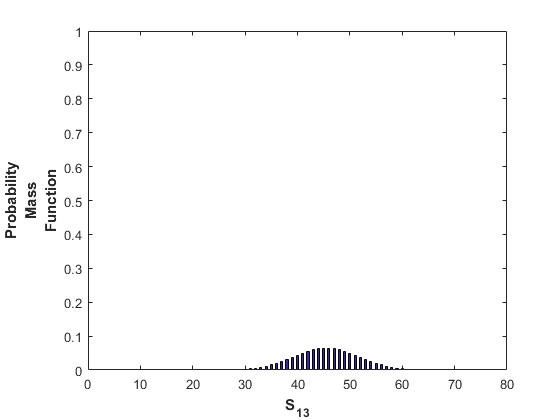
\includegraphics[width=\textwidth]{./Images/7/13.png}
			\caption{ $n=13$ }
		\end{subfigure}
	
		\begin{subfigure}[h!]{0.48\textwidth}
			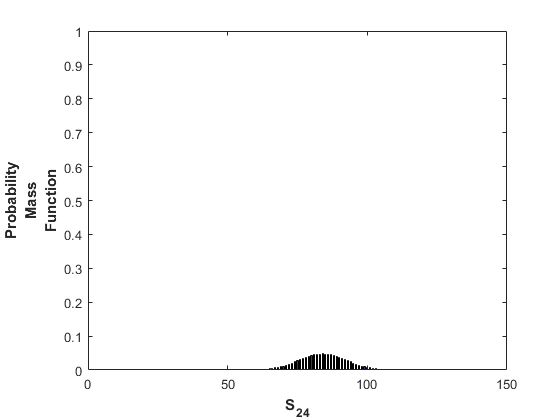
\includegraphics[width=\textwidth]{./Images/7/24.png}
			\caption{ $n=24$ }
		\end{subfigure}
		\quad
		\begin{subfigure}[h!]{0.48\textwidth}
			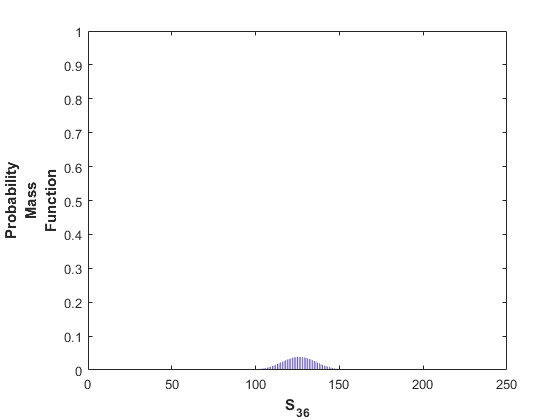
\includegraphics[width=\textwidth]{./Images/7/36.png}
			\caption{ $n=36$ }
		\end{subfigure}
		\caption{نمودار‌های پرسش ۷}
		\label{q7}
	\end{figure}
\end{document}